\documentclass[12pt]{article} 
\usepackage[utf8]{inputenc}
\usepackage{geometry}
\geometry{letterpaper}
\usepackage{graphicx} 
\usepackage{parskip}
\usepackage{booktabs}
\usepackage{array} 
\usepackage{paralist} 
\usepackage{verbatim}
\usepackage{subfig}
\usepackage{fancyhdr}
\usepackage{sectsty}
\usepackage{mathtools}
\usepackage{empheq}
\pagestyle{fancy}
\renewcommand{\headrulewidth}{0pt} 
\lhead{}\chead{}\rhead{}
\lfoot{}\cfoot{\thepage}\rfoot{}

%%% SECTION TITLE APPEARANCE
\allsectionsfont{\sffamily\mdseries\upshape} 

%%% ToC (table of contents) APPEARANCE
\usepackage[nottoc,notlof,notlot]{tocbibind} 
\usepackage[titles,subfigure]{tocloft}
\renewcommand{\cftsecfont}{\rmfamily\mdseries\upshape}
\renewcommand{\cftsecpagefont}{\rmfamily\mdseries\upshape} %

\usepackage{amsmath}
\usepackage{amssymb}

\title{APMA 0350: Homework 9}
\author{Milan Capoor}
\date{18 November 2022}

\begin{document}
\maketitle
\textbf{Problem 1:} Find the general solutions
\begin{enumerate}
    \item $y'' + 6y' + 25y = 0$
    
    Solution:
    \[r^2 + 6r + 25 = 0\]
    \[r = \frac{-6 \pm \sqrt{36 - 4(25)}}{2} = -3 \pm 4i\]
    \[\boxed{y = Ae^{-3t} \cos (4t) + Be^{-3t} \sin (4t)} \] 

    \item $4y'' + 4y' + y = 0$
    
    Solution:
    \[4r^2 + 4r + 1 = 0 \implies (2r + 1)^2 = 0 \implies r = -\frac{1}{2}\]
    \[\boxed{y = Ae^{-t/2} + Bte^{-t/2}}\]

    \item An ODE with Aux equation 
    \[5r^2 (r + 4)^3 (r + 7)(r^2 + 9)^3 (r^2 + 2r + 10)^2 = 0\]
    Solution:
    \[r = \{0, \; -4, \; -7\; \pm 3i,\; -1 \pm 3i\}\]
    \begin{empheq}[box=\fbox]{align*}
        & y = 1 + Ae^{-4t} + Bte^{-4t} + Ct^2e^{-4t} + De^{-7t} + E\cos(3t)\\ 
        & + F\cos(3t) + Gt\cos(3t) + Ht\cos(3t) + It^2 \cos(3t) + Jt^2 \cos(3t) \\
        &+ Ke^{-t}\cos(3t) + Le^{-t} \sin(3t) + Mte^{-t}\cos(3t)+ Nte^{-t} \sin(3t)
    \end{empheq}
\end{enumerate}

\textbf{Problem 2:} Solve the ODE
\[\begin{cases}
    y'' - 6y' + 13y = 0\\
    y(0) = 2\\
    y'(0) = 10
\end{cases}\]

Solution:
\[r^2 - 6r + 13 = 0\]
\[r = \frac{6 \pm \sqrt{36 - 52}}{2} = 3 \pm 2i\]
\[y = Ae^{3t} \cos(2t) + Be^{3t} \sin(2t)\]
\[y(0) = A = 2\]
\[y' = 3Ae^{3t} \cos (2t) -2Ae^{3t} \sin (2t) + 3Be^{3t} \sin (2t) + 2Be^{3t} \cos (2t)\]
\[y'(0) = 3A + 2B = 10 = 6 + 2B \implies B = 2\]
\[\boxed{y = 2e^{3t} \cos(2t) + 2e^{3t} \sin(2t)}\]

\pagebreak 

\textbf{Problem 3:} Find the eigenvalues and eigenfunctions of 
\[\begin{cases}
    y'' = \lambda y\\
    y'(0) = 0\\
    y(3) = 0
\end{cases}\]

Aux equation: 
\[r^2 = \lambda\]

Cases:
\begin{enumerate}
    \item $\lambda > 0$
    Then, $\lambda = \omega^2$ for some $\omega > 0$
    \[r^2 = \lambda = \omega^2 \implies r = \pm \omega\]
    \[y = Ae^{\omega t} + Be^{-\omega t}\]
    \[y(3) = Ae^{3\omega} + Be^{-3\omega} = 0\]
    \[y' = \omega Ae^{\omega t} - \omega Be^{- \omega t}\]
    \[y'(0) = A\omega - B\omega = 0 \implies A = B\]
    \[y = Ae^{3\omega} + Ae^{-3\omega} = 0 \]
    Searching for a nonzero solution and dividing through by $Ae^\omega$:
    \[\implies e^3 + e^{-3} = 0\]
    But this is not true so there are no nonzero solutions for $\lambda > 0$
    
    \item $\lambda = 0$
    \[y = A + Bt\]
    \[y'(0) = B = 0\]
    \[y(3) = A = 0\]
    \[y = 0\]
    So there are no nonzero solutions for $\lambda = 0$

    \item $\lambda < 0$
    \[r^2 = \lambda = -\omega^2 \implies r = \pm \omega i \quad (\omega > 0)\]
    \[y = A\cos(\omega t) + B \sin(\omega t)\]
    \[y' = -A\omega \sin(\omega t) + B\omega \cos( \omega t)\]
    \[y' (0) = B\omega = 0 \implies B = 0 \]
    \[y(3) = A\cos(3\omega) = 0\]
    \[\cos(3\omega) = 0\]
    \[3\omega = \frac{\pi}{2} + \pi m\]
    \[\omega = \frac{\pi}{6} + \frac{\pi}{3} m \quad (m \in \mathbb{N}_0)\]
\end{enumerate}

So, 
Eigenvalues: 
\[\lambda = -\omega^2 = \boxed{-\left(\frac{\pi}{6} + \frac{\pi}{3}m\right)^2 \quad (m \in \mathbb{N}_0)}\]
Eigenfunctions:
\[\boxed{y = \cos(\left(\frac{\pi}{6} + \frac{\pi}{3} m\right)t) \quad (m \in \mathbb{N}_0)}\]

\pagebreak

\textbf{Problem 4:} Use undetermined coefficients to solve
\[\begin{cases}
    y'' - 5y' + 4y = 20\cos (2t) + 30\sin (2t)\\
    y(0) = 1\\
    y'(0) = 3
\end{cases}\]

Homogeneous solution:
\[r^2 - 5r + 4 = 0 \implies (r - 4)(r- 1) = \implies r = \{1, 4\}\]
\[y_0 = Ae^t + Be^{4t}\]

Particular solution:
\[20 \cos(2t) + 30\sin(2t) = 0 \implies r = 2i\]

There is no resonance so:
\[y_p = A\cos(2t) + B\sin(2t) + C\cos(2t) + D\sin(2t) = A\cos(2t) + B\sin(2t)\]

\[(A\cos(2t) + B\sin(2t))'' - 5(A\cos(2t) + B\sin(2t))' + 4(A\cos(2t) + B\sin(2t))\]
\[= 20\cos(2t) + 30\sin(2t)\]

\[-4A\cos(2t) - 4B\sin(2t) + 10A\sin(2t) - 10B\cos(2t) + 4A\cos(2t) + 4B\sin(2t)\] 
\[= 20\cos(2t) + 30\sin(2t)\]

\[(-4A - 10B + 4A) \cos(2t) + (-4B + 10A + 4B) \sin(2t) = 20\cos(2t) + 30\sin(2t)\]
\[\begin{cases}
    -10B = 20\\
    10A = 30
\end{cases} \implies A = 3, \quad B = -2\]
\[y_p = 3\cos(2t) - 2\sin(2t)\]

General solution:
\[y = Ae^t + Be^{4t} + 3\cos(2t) - 2\sin(2t)\]
\[y(0) = A + B + 3 = 1\]
\[y' = Ae^t + 4Be^t - 6\sin(2t) - 4\cos(t)\]
\[y'(0) = A + 4B - 4 = 3\]
\[\begin{cases}
    A + B = -2\\
    A + 4B = 7
\end{cases}\]
\[(7 -4B) + B = -2 \implies B = 3 \implies A = -5\]
\[\boxed{y = -5e^t + 3e^{4t} + 3\cos(2t) - 2\sin(2t)}\]

\pagebreak 

\textbf{Problem 5:} Guess the form of the particular solution
\begin{enumerate}
    \item $y'' - 3y' + 2y$
    Aux equation:
    \[r^2 - 3r + 2 = 0 \implies r =\{1, 2\}\]
    There is resonance so the form of the particular solution is 
    \[\boxed{Ate^t}\]

    \item $y'' - 3y' + 2y = t^2e ^{2t}$
    There is also resonance here so the particular solution is 
    \[\boxed{t(At^2 + Bt + C)e^{2t}}\]

    \item $y'' - 2y' + 5y = \sin(2t)$
    Aux equation: 
    \[r^2 - 2r + 5 \implies r = \frac{2 \pm \sqrt{4 - 20}}{2} = 1 \pm 2i\]
    No resonance so the form of $y_p$ is 
    \[\boxed{A\cos(2t) + B\sin(2t)}\]

    \item $y'' - 2y' + 5y = e^t\cos(2t)$
    There is no resonance so the form of $y_p$ is 
    \[\boxed{Ae^t \cos(2t) + Be^t\sin(2t)}\]
\end{enumerate}

\pagebreak 

\textbf{Problem 6:} Use the dsolve command in Python to solve the following ODE. Please
include a screenshot of your code and your solution/plot.
\begin{enumerate}
    \item Solve but do not plot
    \[2y'' + 4y' + y = 0\]

    Solution:

    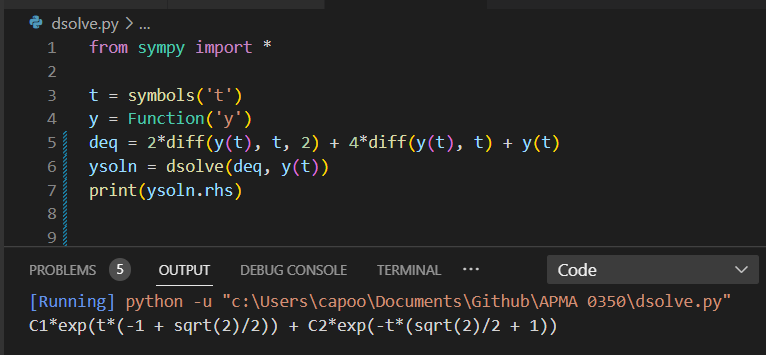
\includegraphics{Images/5a code.png}

    \item Solve and plot for $-20 \leq t \leq 1$
    \[\begin{cases}
        y'' + 4y = 2e^{3t} + 2t + 6\cos t\\
        y(0) = 1\\
        y'(0) = 1
    \end{cases}\]

    Solution:
\end{enumerate}

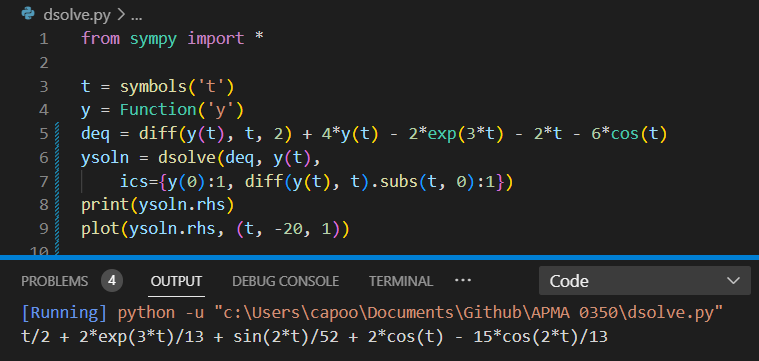
\includegraphics[width=0.6\textwidth]{Images/5b code.png}
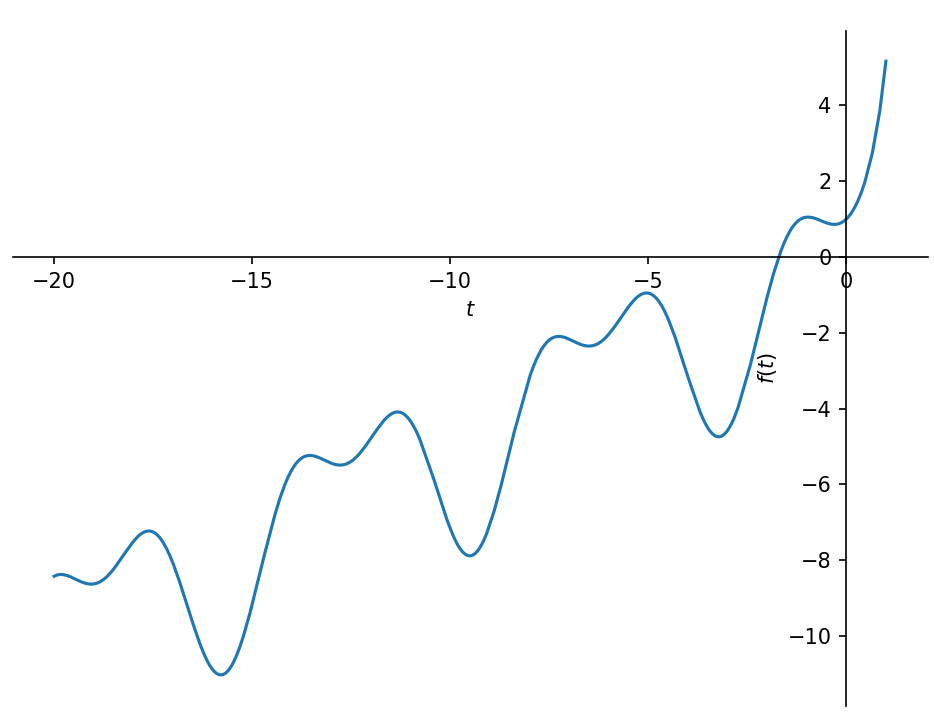
\includegraphics[width=0.4\textwidth]{Images/5b plot.png}
\end{document}